%% ============================================================================
%% Target journal : Journal of Biomedical Informatics (Elsevier, Q1)
%% Template       : elsarticle (available natively on Overleaf)
%% Compile        : pdflatex -> bibtex -> pdflatex x2   (Overleaf: automatic)
%% Results macros : tables/numbers.tex is regenerated by
%%                  M2MIAS/simulations/make_figures.py --latex <this folder>
%% ============================================================================
\documentclass[preprint,12pt]{elsarticle}

\usepackage[T1]{fontenc}
\usepackage[utf8]{inputenc}
\usepackage{lmodern}
\usepackage{amsmath,amssymb,amsthm}
\usepackage{graphicx}
\usepackage{booktabs}
\usepackage{multirow}
\usepackage{xcolor}
\usepackage[a4paper,margin=2.5cm]{geometry}
\usepackage{hyperref}
\usepackage[capitalise,noabbrev]{cleveref}
\usepackage{lineno}
%\linenumbers   % uncomment for submission

\hypersetup{colorlinks=true,linkcolor=blue!50!black,citecolor=blue!50!black,urlcolor=blue!50!black}
\graphicspath{{figures/}}
\newtheorem{proposition}{Proposition}
\newtheorem{definition}{Definition}
\newcommand{\kL}{\kappa_{L}}
\newcommand{\G}{G29}

\newcommand{\Nrec}{1500}
\newcommand{\Norders}{30}
\newcommand{\kmaxA}{17}
\newcommand{\kmaxB}{13}
\newcommand{\UniqDirZero}{1.00}
\newcommand{\PpvDirZero}{1.00}
\newcommand{\LinkExDirZero}{1.00}
\newcommand{\LinkNNDirZero}{1.00}
\newcommand{\KappaDirZero}{1.00}
\newcommand{\UniqPeakDirZero}{1.00}
\newcommand{\AukcDirZero}{0.59}
\newcommand{\InfDemAccDirZero}{1.00}
\newcommand{\InfDemMccDirZero}{1.00}
\newcommand{\InfDemBaDirZero}{1.00}
\newcommand{\InfDemApDirZero}{1.00}
\newcommand{\InfDemAccGainDirZero}{1.00}
\newcommand{\InfDemPrevDirZero}{0.04}
\newcommand{\InfDiaAccDirZero}{1.00}
\newcommand{\InfDiaMccDirZero}{1.00}
\newcommand{\InfDiaBaDirZero}{1.00}
\newcommand{\InfDiaApDirZero}{1.00}
\newcommand{\InfDiaAccGainDirZero}{1.00}
\newcommand{\InfDiaPrevDirZero}{0.13}
\newcommand{\InfRenAccDirZero}{1.00}
\newcommand{\InfRenMccDirZero}{1.00}
\newcommand{\InfRenBaDirZero}{1.00}
\newcommand{\InfRenApDirZero}{1.00}
\newcommand{\InfRenAccGainDirZero}{1.00}
\newcommand{\InfRenPrevDirZero}{0.06}
\newcommand{\InfChiAccDirZero}{1.00}
\newcommand{\InfChiMccDirZero}{1.00}
\newcommand{\InfChiBaDirZero}{1.00}
\newcommand{\InfChiApDirZero}{1.00}
\newcommand{\InfChiAccGainDirZero}{1.00}
\newcommand{\InfChiPrevDirZero}{0.29}
\newcommand{\UniqDirTen}{0.31}
\newcommand{\PpvDirTen}{1.00}
\newcommand{\LinkExDirTen}{0.31}
\newcommand{\LinkNNDirTen}{0.99}
\newcommand{\KappaDirTen}{0.99}
\newcommand{\UniqPeakDirTen}{0.48}
\newcommand{\AukcDirTen}{0.51}
\newcommand{\InfDemAccDirTen}{0.99}
\newcommand{\InfDemMccDirTen}{0.89}
\newcommand{\InfDemBaDirTen}{0.95}
\newcommand{\InfDemApDirTen}{0.82}
\newcommand{\InfDemAccGainDirTen}{0.79}
\newcommand{\InfDemPrevDirTen}{0.04}
\newcommand{\InfDiaAccDirTen}{0.97}
\newcommand{\InfDiaMccDirTen}{0.88}
\newcommand{\InfDiaBaDirTen}{0.94}
\newcommand{\InfDiaApDirTen}{0.82}
\newcommand{\InfDiaAccGainDirTen}{0.79}
\newcommand{\InfDiaPrevDirTen}{0.13}
\newcommand{\InfRenAccDirTen}{0.99}
\newcommand{\InfRenMccDirTen}{0.86}
\newcommand{\InfRenBaDirTen}{0.93}
\newcommand{\InfRenApDirTen}{0.75}
\newcommand{\InfRenAccGainDirTen}{0.74}
\newcommand{\InfRenPrevDirTen}{0.06}
\newcommand{\InfChiAccDirTen}{0.96}
\newcommand{\InfChiMccDirTen}{0.90}
\newcommand{\InfChiBaDirTen}{0.95}
\newcommand{\InfChiApDirTen}{0.84}
\newcommand{\InfChiAccGainDirTen}{0.85}
\newcommand{\InfChiPrevDirTen}{0.29}
\newcommand{\UniqDirTwentyFive}{0.05}
\newcommand{\PpvDirTwentyFive}{1.00}
\newcommand{\LinkExDirTwentyFive}{0.05}
\newcommand{\LinkNNDirTwentyFive}{0.89}
\newcommand{\KappaDirTwentyFive}{0.89}
\newcommand{\UniqPeakDirTwentyFive}{0.30}
\newcommand{\AukcDirTwentyFive}{0.38}
\newcommand{\InfDemAccDirTwentyFive}{0.98}
\newcommand{\InfDemMccDirTwentyFive}{0.77}
\newcommand{\InfDemBaDirTwentyFive}{0.87}
\newcommand{\InfDemApDirTwentyFive}{0.63}
\newcommand{\InfDemAccGainDirTwentyFive}{0.57}
\newcommand{\InfDemPrevDirTwentyFive}{0.04}
\newcommand{\InfDiaAccDirTwentyFive}{0.92}
\newcommand{\InfDiaMccDirTwentyFive}{0.65}
\newcommand{\InfDiaBaDirTwentyFive}{0.83}
\newcommand{\InfDiaApDirTwentyFive}{0.51}
\newcommand{\InfDiaAccGainDirTwentyFive}{0.39}
\newcommand{\InfDiaPrevDirTwentyFive}{0.13}
\newcommand{\InfRenAccDirTwentyFive}{0.97}
\newcommand{\InfRenMccDirTwentyFive}{0.74}
\newcommand{\InfRenBaDirTwentyFive}{0.87}
\newcommand{\InfRenApDirTwentyFive}{0.62}
\newcommand{\InfRenAccGainDirTwentyFive}{0.50}
\newcommand{\InfRenPrevDirTwentyFive}{0.06}
\newcommand{\InfChiAccDirTwentyFive}{0.89}
\newcommand{\InfChiMccDirTwentyFive}{0.73}
\newcommand{\InfChiBaDirTwentyFive}{0.87}
\newcommand{\InfChiApDirTwentyFive}{0.62}
\newcommand{\InfChiAccGainDirTwentyFive}{0.62}
\newcommand{\InfChiPrevDirTwentyFive}{0.29}
\newcommand{\UniqDirFifty}{0.00}
\newcommand{\PpvDirFifty}{1.00}
\newcommand{\LinkExDirFifty}{0.00}
\newcommand{\LinkNNDirFifty}{0.52}
\newcommand{\KappaDirFifty}{0.52}
\newcommand{\UniqPeakDirFifty}{0.18}
\newcommand{\AukcDirFifty}{0.18}
\newcommand{\InfDemAccDirFifty}{0.95}
\newcommand{\InfDemMccDirFifty}{0.43}
\newcommand{\InfDemBaDirFifty}{0.70}
\newcommand{\InfDemApDirFifty}{0.24}
\newcommand{\InfDemAccGainDirFifty}{-0.06}
\newcommand{\InfDemPrevDirFifty}{0.04}
\newcommand{\InfDiaAccDirFifty}{0.83}
\newcommand{\InfDiaMccDirFifty}{0.26}
\newcommand{\InfDiaBaDirFifty}{0.63}
\newcommand{\InfDiaApDirFifty}{0.13}
\newcommand{\InfDiaAccGainDirFifty}{-0.27}
\newcommand{\InfDiaPrevDirFifty}{0.13}
\newcommand{\InfRenAccDirFifty}{0.93}
\newcommand{\InfRenMccDirFifty}{0.35}
\newcommand{\InfRenBaDirFifty}{0.67}
\newcommand{\InfRenApDirFifty}{0.17}
\newcommand{\InfRenAccGainDirFifty}{-0.18}
\newcommand{\InfRenPrevDirFifty}{0.06}
\newcommand{\InfChiAccDirFifty}{0.74}
\newcommand{\InfChiMccDirFifty}{0.36}
\newcommand{\InfChiBaDirFifty}{0.68}
\newcommand{\InfChiApDirFifty}{0.27}
\newcommand{\InfChiAccGainDirFifty}{0.09}
\newcommand{\InfChiPrevDirFifty}{0.29}
\newcommand{\UniqDirSeventyFive}{0.00}
\newcommand{\PpvDirSeventyFive}{nan}
\newcommand{\LinkExDirSeventyFive}{0.00}
\newcommand{\LinkNNDirSeventyFive}{0.13}
\newcommand{\KappaDirSeventyFive}{0.13}
\newcommand{\UniqPeakDirSeventyFive}{0.15}
\newcommand{\AukcDirSeventyFive}{0.04}
\newcommand{\InfDemAccDirSeventyFive}{0.92}
\newcommand{\InfDemMccDirSeventyFive}{0.04}
\newcommand{\InfDemBaDirSeventyFive}{0.52}
\newcommand{\InfDemApDirSeventyFive}{0.01}
\newcommand{\InfDemAccGainDirSeventyFive}{-0.79}
\newcommand{\InfDemPrevDirSeventyFive}{0.04}
\newcommand{\InfDiaAccDirSeventyFive}{0.80}
\newcommand{\InfDiaMccDirSeventyFive}{0.03}
\newcommand{\InfDiaBaDirSeventyFive}{0.52}
\newcommand{\InfDiaApDirSeventyFive}{0.01}
\newcommand{\InfDiaAccGainDirSeventyFive}{-0.54}
\newcommand{\InfDiaPrevDirSeventyFive}{0.13}
\newcommand{\InfRenAccDirSeventyFive}{0.90}
\newcommand{\InfRenMccDirSeventyFive}{-0.01}
\newcommand{\InfRenBaDirSeventyFive}{0.50}
\newcommand{\InfRenApDirSeventyFive}{0.00}
\newcommand{\InfRenAccGainDirSeventyFive}{-0.87}
\newcommand{\InfRenPrevDirSeventyFive}{0.06}
\newcommand{\InfChiAccDirSeventyFive}{0.62}
\newcommand{\InfChiMccDirSeventyFive}{0.10}
\newcommand{\InfChiBaDirSeventyFive}{0.55}
\newcommand{\InfChiApDirSeventyFive}{0.06}
\newcommand{\InfChiAccGainDirSeventyFive}{-0.32}
\newcommand{\InfChiPrevDirSeventyFive}{0.29}
\newcommand{\UniqDirNinety}{0.00}
\newcommand{\PpvDirNinety}{nan}
\newcommand{\LinkExDirNinety}{0.00}
\newcommand{\LinkNNDirNinety}{0.01}
\newcommand{\KappaDirNinety}{0.01}
\newcommand{\UniqPeakDirNinety}{0.14}
\newcommand{\AukcDirNinety}{0.00}
\newcommand{\InfDemAccDirNinety}{0.91}
\newcommand{\InfDemMccDirNinety}{-0.00}
\newcommand{\InfDemBaDirNinety}{0.50}
\newcommand{\InfDemApDirNinety}{0.00}
\newcommand{\InfDemAccGainDirNinety}{-0.93}
\newcommand{\InfDemPrevDirNinety}{0.04}
\newcommand{\InfDiaAccDirNinety}{0.79}
\newcommand{\InfDiaMccDirNinety}{-0.04}
\newcommand{\InfDiaBaDirNinety}{0.48}
\newcommand{\InfDiaApDirNinety}{-0.01}
\newcommand{\InfDiaAccGainDirNinety}{-0.58}
\newcommand{\InfDiaPrevDirNinety}{0.13}
\newcommand{\InfRenAccDirNinety}{0.90}
\newcommand{\InfRenMccDirNinety}{-0.02}
\newcommand{\InfRenBaDirNinety}{0.49}
\newcommand{\InfRenApDirNinety}{-0.00}
\newcommand{\InfRenAccGainDirNinety}{-0.82}
\newcommand{\InfRenPrevDirNinety}{0.06}
\newcommand{\InfChiAccDirNinety}{0.60}
\newcommand{\InfChiMccDirNinety}{-0.00}
\newcommand{\InfChiBaDirNinety}{0.50}
\newcommand{\InfChiApDirNinety}{0.02}
\newcommand{\InfChiAccGainDirNinety}{-0.38}
\newcommand{\InfChiPrevDirNinety}{0.29}
\newcommand{\UniqDirHundred}{0.00}
\newcommand{\PpvDirHundred}{nan}
\newcommand{\LinkExDirHundred}{0.00}
\newcommand{\LinkNNDirHundred}{0.00}
\newcommand{\KappaDirHundred}{0.00}
\newcommand{\UniqPeakDirHundred}{0.15}
\newcommand{\AukcDirHundred}{0.00}
\newcommand{\InfDemAccDirHundred}{0.93}
\newcommand{\InfDemMccDirHundred}{0.04}
\newcommand{\InfDemBaDirHundred}{0.52}
\newcommand{\InfDemApDirHundred}{0.01}
\newcommand{\InfDemAccGainDirHundred}{-0.49}
\newcommand{\InfDemPrevDirHundred}{0.04}
\newcommand{\InfDiaAccDirHundred}{0.79}
\newcommand{\InfDiaMccDirHundred}{-0.01}
\newcommand{\InfDiaBaDirHundred}{0.50}
\newcommand{\InfDiaApDirHundred}{-0.00}
\newcommand{\InfDiaAccGainDirHundred}{-0.60}
\newcommand{\InfDiaPrevDirHundred}{0.13}
\newcommand{\InfRenAccDirHundred}{0.91}
\newcommand{\InfRenMccDirHundred}{0.03}
\newcommand{\InfRenBaDirHundred}{0.51}
\newcommand{\InfRenApDirHundred}{0.01}
\newcommand{\InfRenAccGainDirHundred}{-0.64}
\newcommand{\InfRenPrevDirHundred}{0.06}
\newcommand{\InfChiAccDirHundred}{0.60}
\newcommand{\InfChiMccDirHundred}{-0.01}
\newcommand{\InfChiBaDirHundred}{0.50}
\newcommand{\InfChiApDirHundred}{-0.01}
\newcommand{\InfChiAccGainDirHundred}{-0.40}
\newcommand{\InfChiPrevDirHundred}{0.29}
\newcommand{\CeilDir}{1.00}
\newcommand{\UniqSmpZero}{0.36}
\newcommand{\PpvSmpZero}{1.00}
\newcommand{\LinkExSmpZero}{0.63}
\newcommand{\LinkNNSmpZero}{0.63}
\newcommand{\KappaSmpZero}{1.00}
\newcommand{\UniqPeakSmpZero}{0.36}
\newcommand{\AukcSmpZero}{0.61}
\newcommand{\InfDemAccSmpZero}{0.97}
\newcommand{\InfDemMccSmpZero}{0.68}
\newcommand{\InfDemBaSmpZero}{0.82}
\newcommand{\InfDemApSmpZero}{0.56}
\newcommand{\InfDemAccGainSmpZero}{0.42}
\newcommand{\InfDemPrevSmpZero}{0.04}
\newcommand{\InfDiaAccSmpZero}{0.92}
\newcommand{\InfDiaMccSmpZero}{0.64}
\newcommand{\InfDiaBaSmpZero}{0.80}
\newcommand{\InfDiaApSmpZero}{0.51}
\newcommand{\InfDiaAccGainSmpZero}{0.40}
\newcommand{\InfDiaPrevSmpZero}{0.13}
\newcommand{\InfRenAccSmpZero}{0.96}
\newcommand{\InfRenMccSmpZero}{0.66}
\newcommand{\InfRenBaSmpZero}{0.82}
\newcommand{\InfRenApSmpZero}{0.52}
\newcommand{\InfRenAccGainSmpZero}{0.37}
\newcommand{\InfRenPrevSmpZero}{0.06}
\newcommand{\InfChiAccSmpZero}{0.91}
\newcommand{\InfChiMccSmpZero}{0.78}
\newcommand{\InfChiBaSmpZero}{0.89}
\newcommand{\InfChiApSmpZero}{0.77}
\newcommand{\InfChiAccGainSmpZero}{0.70}
\newcommand{\InfChiPrevSmpZero}{0.29}
\newcommand{\UniqSmpTen}{0.23}
\newcommand{\PpvSmpTen}{1.00}
\newcommand{\LinkExSmpTen}{0.28}
\newcommand{\LinkNNSmpTen}{0.61}
\newcommand{\KappaSmpTen}{0.99}
\newcommand{\UniqPeakSmpTen}{0.31}
\newcommand{\AukcSmpTen}{0.56}
\newcommand{\InfDemAccSmpTen}{0.97}
\newcommand{\InfDemMccSmpTen}{0.71}
\newcommand{\InfDemBaSmpTen}{0.87}
\newcommand{\InfDemApSmpTen}{0.65}
\newcommand{\InfDemAccGainSmpTen}{0.42}
\newcommand{\InfDemPrevSmpTen}{0.04}
\newcommand{\InfDiaAccSmpTen}{0.90}
\newcommand{\InfDiaMccSmpTen}{0.55}
\newcommand{\InfDiaBaSmpTen}{0.78}
\newcommand{\InfDiaApSmpTen}{0.46}
\newcommand{\InfDiaAccGainSmpTen}{0.22}
\newcommand{\InfDiaPrevSmpTen}{0.13}
\newcommand{\InfRenAccSmpTen}{0.96}
\newcommand{\InfRenMccSmpTen}{0.64}
\newcommand{\InfRenBaSmpTen}{0.83}
\newcommand{\InfRenApSmpTen}{0.53}
\newcommand{\InfRenAccGainSmpTen}{0.30}
\newcommand{\InfRenPrevSmpTen}{0.06}
\newcommand{\InfChiAccSmpTen}{0.88}
\newcommand{\InfChiMccSmpTen}{0.72}
\newcommand{\InfChiBaSmpTen}{0.86}
\newcommand{\InfChiApSmpTen}{0.66}
\newcommand{\InfChiAccGainSmpTen}{0.60}
\newcommand{\InfChiPrevSmpTen}{0.29}
\newcommand{\UniqSmpTwentyFive}{0.05}
\newcommand{\PpvSmpTwentyFive}{1.00}
\newcommand{\LinkExSmpTwentyFive}{0.05}
\newcommand{\LinkNNSmpTwentyFive}{0.60}
\newcommand{\KappaSmpTwentyFive}{0.94}
\newcommand{\UniqPeakSmpTwentyFive}{0.25}
\newcommand{\AukcSmpTwentyFive}{0.44}
\newcommand{\InfDemAccSmpTwentyFive}{0.95}
\newcommand{\InfDemMccSmpTwentyFive}{0.50}
\newcommand{\InfDemBaSmpTwentyFive}{0.77}
\newcommand{\InfDemApSmpTwentyFive}{0.42}
\newcommand{\InfDemAccGainSmpTwentyFive}{-0.03}
\newcommand{\InfDemPrevSmpTwentyFive}{0.04}
\newcommand{\InfDiaAccSmpTwentyFive}{0.87}
\newcommand{\InfDiaMccSmpTwentyFive}{0.44}
\newcommand{\InfDiaBaSmpTwentyFive}{0.72}
\newcommand{\InfDiaApSmpTwentyFive}{0.29}
\newcommand{\InfDiaAccGainSmpTwentyFive}{0.04}
\newcommand{\InfDiaPrevSmpTwentyFive}{0.13}
\newcommand{\InfRenAccSmpTwentyFive}{0.94}
\newcommand{\InfRenMccSmpTwentyFive}{0.48}
\newcommand{\InfRenBaSmpTwentyFive}{0.75}
\newcommand{\InfRenApSmpTwentyFive}{0.30}
\newcommand{\InfRenAccGainSmpTwentyFive}{0.00}
\newcommand{\InfRenPrevSmpTwentyFive}{0.06}
\newcommand{\InfChiAccSmpTwentyFive}{0.80}
\newcommand{\InfChiMccSmpTwentyFive}{0.53}
\newcommand{\InfChiBaSmpTwentyFive}{0.77}
\newcommand{\InfChiApSmpTwentyFive}{0.44}
\newcommand{\InfChiAccGainSmpTwentyFive}{0.32}
\newcommand{\InfChiPrevSmpTwentyFive}{0.29}
\newcommand{\UniqSmpFifty}{0.00}
\newcommand{\PpvSmpFifty}{1.00}
\newcommand{\LinkExSmpFifty}{0.00}
\newcommand{\LinkNNSmpFifty}{0.38}
\newcommand{\KappaSmpFifty}{0.61}
\newcommand{\UniqPeakSmpFifty}{0.17}
\newcommand{\AukcSmpFifty}{0.23}
\newcommand{\InfDemAccSmpFifty}{0.94}
\newcommand{\InfDemMccSmpFifty}{0.20}
\newcommand{\InfDemBaSmpFifty}{0.58}
\newcommand{\InfDemApSmpFifty}{0.08}
\newcommand{\InfDemAccGainSmpFifty}{-0.27}
\newcommand{\InfDemPrevSmpFifty}{0.04}
\newcommand{\InfDiaAccSmpFifty}{0.83}
\newcommand{\InfDiaMccSmpFifty}{0.22}
\newcommand{\InfDiaBaSmpFifty}{0.61}
\newcommand{\InfDiaApSmpFifty}{0.11}
\newcommand{\InfDiaAccGainSmpFifty}{-0.29}
\newcommand{\InfDiaPrevSmpFifty}{0.13}
\newcommand{\InfRenAccSmpFifty}{0.94}
\newcommand{\InfRenMccSmpFifty}{0.36}
\newcommand{\InfRenBaSmpFifty}{0.66}
\newcommand{\InfRenApSmpFifty}{0.18}
\newcommand{\InfRenAccGainSmpFifty}{-0.13}
\newcommand{\InfRenPrevSmpFifty}{0.06}
\newcommand{\InfChiAccSmpFifty}{0.74}
\newcommand{\InfChiMccSmpFifty}{0.37}
\newcommand{\InfChiBaSmpFifty}{0.69}
\newcommand{\InfChiApSmpFifty}{0.26}
\newcommand{\InfChiAccGainSmpFifty}{0.08}
\newcommand{\InfChiPrevSmpFifty}{0.29}
\newcommand{\UniqSmpSeventyFive}{0.00}
\newcommand{\PpvSmpSeventyFive}{nan}
\newcommand{\LinkExSmpSeventyFive}{0.00}
\newcommand{\LinkNNSmpSeventyFive}{0.11}
\newcommand{\KappaSmpSeventyFive}{0.19}
\newcommand{\UniqPeakSmpSeventyFive}{0.15}
\newcommand{\AukcSmpSeventyFive}{0.06}
\newcommand{\InfDemAccSmpSeventyFive}{0.94}
\newcommand{\InfDemMccSmpSeventyFive}{0.05}
\newcommand{\InfDemBaSmpSeventyFive}{0.52}
\newcommand{\InfDemApSmpSeventyFive}{0.01}
\newcommand{\InfDemAccGainSmpSeventyFive}{-0.45}
\newcommand{\InfDemPrevSmpSeventyFive}{0.04}
\newcommand{\InfDiaAccSmpSeventyFive}{0.81}
\newcommand{\InfDiaMccSmpSeventyFive}{0.10}
\newcommand{\InfDiaBaSmpSeventyFive}{0.54}
\newcommand{\InfDiaApSmpSeventyFive}{0.04}
\newcommand{\InfDiaAccGainSmpSeventyFive}{-0.44}
\newcommand{\InfDiaPrevSmpSeventyFive}{0.13}
\newcommand{\InfRenAccSmpSeventyFive}{0.91}
\newcommand{\InfRenMccSmpSeventyFive}{0.01}
\newcommand{\InfRenBaSmpSeventyFive}{0.51}
\newcommand{\InfRenApSmpSeventyFive}{0.00}
\newcommand{\InfRenAccGainSmpSeventyFive}{-0.58}
\newcommand{\InfRenPrevSmpSeventyFive}{0.06}
\newcommand{\InfChiAccSmpSeventyFive}{0.62}
\newcommand{\InfChiMccSmpSeventyFive}{0.04}
\newcommand{\InfChiBaSmpSeventyFive}{0.52}
\newcommand{\InfChiApSmpSeventyFive}{0.04}
\newcommand{\InfChiAccGainSmpSeventyFive}{-0.33}
\newcommand{\InfChiPrevSmpSeventyFive}{0.29}
\newcommand{\UniqSmpNinety}{0.00}
\newcommand{\PpvSmpNinety}{nan}
\newcommand{\LinkExSmpNinety}{0.00}
\newcommand{\LinkNNSmpNinety}{0.01}
\newcommand{\KappaSmpNinety}{0.02}
\newcommand{\UniqPeakSmpNinety}{0.16}
\newcommand{\AukcSmpNinety}{0.01}
\newcommand{\InfDemAccSmpNinety}{0.93}
\newcommand{\InfDemMccSmpNinety}{0.02}
\newcommand{\InfDemBaSmpNinety}{0.51}
\newcommand{\InfDemApSmpNinety}{0.00}
\newcommand{\InfDemAccGainSmpNinety}{-0.58}
\newcommand{\InfDemPrevSmpNinety}{0.04}
\newcommand{\InfDiaAccSmpNinety}{0.79}
\newcommand{\InfDiaMccSmpNinety}{0.04}
\newcommand{\InfDiaBaSmpNinety}{0.52}
\newcommand{\InfDiaApSmpNinety}{0.01}
\newcommand{\InfDiaAccGainSmpNinety}{-0.59}
\newcommand{\InfDiaPrevSmpNinety}{0.13}
\newcommand{\InfRenAccSmpNinety}{0.91}
\newcommand{\InfRenMccSmpNinety}{0.01}
\newcommand{\InfRenBaSmpNinety}{0.50}
\newcommand{\InfRenApSmpNinety}{0.00}
\newcommand{\InfRenAccGainSmpNinety}{-0.63}
\newcommand{\InfRenPrevSmpNinety}{0.06}
\newcommand{\InfChiAccSmpNinety}{0.59}
\newcommand{\InfChiMccSmpNinety}{0.01}
\newcommand{\InfChiBaSmpNinety}{0.51}
\newcommand{\InfChiApSmpNinety}{0.02}
\newcommand{\InfChiAccGainSmpNinety}{-0.44}
\newcommand{\InfChiPrevSmpNinety}{0.29}
\newcommand{\UniqSmpHundred}{0.00}
\newcommand{\PpvSmpHundred}{nan}
\newcommand{\LinkExSmpHundred}{0.00}
\newcommand{\LinkNNSmpHundred}{0.00}
\newcommand{\KappaSmpHundred}{-0.00}
\newcommand{\UniqPeakSmpHundred}{0.15}
\newcommand{\AukcSmpHundred}{-0.00}
\newcommand{\InfDemAccSmpHundred}{0.92}
\newcommand{\InfDemMccSmpHundred}{-0.01}
\newcommand{\InfDemBaSmpHundred}{0.50}
\newcommand{\InfDemApSmpHundred}{0.00}
\newcommand{\InfDemAccGainSmpHundred}{-0.73}
\newcommand{\InfDemPrevSmpHundred}{0.04}
\newcommand{\InfDiaAccSmpHundred}{0.80}
\newcommand{\InfDiaMccSmpHundred}{0.05}
\newcommand{\InfDiaBaSmpHundred}{0.53}
\newcommand{\InfDiaApSmpHundred}{0.02}
\newcommand{\InfDiaAccGainSmpHundred}{-0.53}
\newcommand{\InfDiaPrevSmpHundred}{0.13}
\newcommand{\InfRenAccSmpHundred}{0.90}
\newcommand{\InfRenMccSmpHundred}{-0.03}
\newcommand{\InfRenBaSmpHundred}{0.49}
\newcommand{\InfRenApSmpHundred}{-0.00}
\newcommand{\InfRenAccGainSmpHundred}{-0.82}
\newcommand{\InfRenPrevSmpHundred}{0.06}
\newcommand{\InfChiAccSmpHundred}{0.60}
\newcommand{\InfChiMccSmpHundred}{0.01}
\newcommand{\InfChiBaSmpHundred}{0.50}
\newcommand{\InfChiApSmpHundred}{0.01}
\newcommand{\InfChiAccGainSmpHundred}{-0.40}
\newcommand{\InfChiPrevSmpHundred}{0.29}
\newcommand{\CeilSmp}{0.63}


\journal{Journal of Biomedical Informatics}

\begin{document}

\begin{frontmatter}

\title{Chance-corrected, imbalance-aware indicators of re-identification risk for synthetic health data: operationalising the singling-out, linkability and inference criteria on knowledge curves}

%% TODO: complete the author list and affiliations before submission.
\author[lab]{Wajdi [Surname]\corref{cor1}}
\ead{[email]}
\cortext[cor1]{Corresponding author.}
\affiliation[lab]{organization={[Laboratory], Master~2 MIAS},
            city={[City]}, country={France}}

\begin{abstract}
\textbf{Objective.} The Article~29 Working Party (\G{}) judges an anonymisation technique on three criteria---singling out, linkability and inference---but does not say how to measure them. Measurements that are routinely used (share of unique records, accuracy of attribute guessing) are biased when the evaluated database is imbalanced: rare diseases, rare discharge modes and bootstrap releases in which a third of the population is absent. We propose and test quantitative indicators for the three criteria that remain interpretable under imbalance.

\textbf{Methods.} We model an adversary who learns a growing number $k$ of a patient's variables, in random orders that respect nested granularities (age, dates). Each released file is attacked by a strict (exact-match) and a tolerant (best-agreement) adversary. We define (i)~the positive predictive value of singling out, (ii)~a chance- and ceiling-corrected linkage index $\kL$, (iii)~inference scores corrected for the majority-class baseline (Matthews correlation coefficient, balanced accuracy, AUPRC gain), (iv)~an excess-risk correction against a maximally perturbed ``null'' release, and (v)~the normalised area under the knowledge curve (nAUKC). Indicators were evaluated on a fictitious hospital-stay database of \Nrec{} stays and on releases obtained by permuting 0--100\% of the cells of each column, with or without bootstrap resampling (\Norders{} random orders).

\textbf{Results.} Naive indicators produced three systematic artefacts. Apparent uniqueness was non-monotone in $k$ and largely spurious on perturbed files (peak \UniqPeakDirHundred{} on a fully shuffled release, with no correct singling out). On the fully shuffled release, raw accuracy for dementia was \InfDemAccDirHundred{}, close to (and below) the trivial majority-class rate, whereas MCC was \InfDemMccDirHundred{}. Exact-match linkage collapsed as soon as cells were shuffled (\LinkExDirTwentyFive{} at 25\% shuffling and full knowledge) while the tolerant adversary still linked \LinkNNDirTwentyFive{} of stays. The corrected indicators decreased with the perturbation level, were close to zero on null releases and were comparable between direct and bootstrap releases.

\textbf{Conclusion.} Risk indicators for synthetic or perturbed health data should be reported as chance-corrected knowledge curves, against a realistic (tolerant) adversary, with imbalance-robust metrics. The proposed set maps one-to-one onto the \G{} criteria and is released as open-source code.
\end{abstract}

\begin{keyword}
Anonymisation \sep re-identification \sep synthetic data \sep GDPR \sep class imbalance \sep Matthews correlation coefficient \sep record linkage \sep privacy metrics
\end{keyword}

\end{frontmatter}

%% ============================================================================
\section{Introduction}
\label{sec:intro}

Sharing hospital data for secondary use requires either a legal basis for processing personal data or a demonstration that the shared data are anonymous in the sense of Recital~26 of the General Data Protection Regulation (GDPR)~\cite{gdpr2016}. In its Opinion 05/2014 on anonymisation techniques~\cite{wp29_2014}, relayed in France by the CNIL~\cite{cnil_g29}, the Article~29 Working Party (\G{}) states that a robust anonymisation must prevent three risks: \emph{singling out} (isolating some or all records that identify an individual), \emph{linkability} (linking at least two records concerning the same individual or group) and \emph{inference} (deducing, with significant probability, the value of an attribute from the values of other attributes). The Opinion is qualitative: it does not say how each risk should be measured, nor what level is acceptable.

Synthetic data generation has become a popular answer to this question, and with it a growing number of privacy metrics~\cite{steier2025metrics,hu2026synqp,pathak2026kde}. Recent work has shown that many of these metrics are unreliable. Similarity-based metrics such as distance to closest record can pass while membership and attribute inference attacks succeed~\cite{ganev2025inadequacy,yao2025dcr}. An international consensus panel recommended focusing on membership and attribute disclosure and avoiding similarity metrics~\cite{pilgram2025consensus}. Controlled risk-insertion experiments show that privacy metrics react unequally to deliberately planted leaks~\cite{plasencia2025empirical}, and fidelity evaluations of synthetic electronic medical records show that marginal resemblance can hide broken dependency structures~\cite{kuo2026synthetic}. Attack-based frameworks such as Anonymeter~\cite{giomi2023anonymeter} operationalise the three \G{} criteria by comparing a ``main'' attack with a control and a naive baseline. Concerns about re-identification in health data keep extending to new data-sharing modalities, such as privacy-preserving record linkage tokens~\cite{eliazar2026pprl}, and synthetic health datasets are now published with explicit anonymity claims~\cite{nanevski2026fall,guillaudeux2023avatar}.

One aspect has received little attention: \textbf{health databases are imbalanced}, and imbalance distorts the most intuitive risk indicators. Imbalance arises at three levels. (1)~\emph{Sensitive attributes} are rare: in a general hospital population, dementia or chronic renal failure concern a few percent of stays. An attacker who always answers ``no'' reaches a high accuracy without learning anything. (2)~\emph{Linkage is a needle-in-a-haystack problem}: for each target exactly one record (or none) out of $M$ is correct, so any pairwise accuracy is dominated by true negatives. (3)~\emph{Presence is imbalanced in resampled releases}: under bootstrap resampling a fraction $(1-1/M)^M \approx e^{-1} \approx 37\%$ of individuals are absent, which caps any success rate at about 63\%. Recent work on classifier evaluation has stressed that accuracy, and to some extent ROC-AUC, are misleading under strong imbalance and has recommended the Matthews correlation coefficient (MCC) and precision--recall summaries~\cite{chicco2020mcc,chicco2023mccroc,saito2015prc,imani2026rocauc}, although the debate on ROC curves is not closed~\cite{richardson2024roc}. To our knowledge these recommendations have not been carried over systematically to re-identification risk indicators.

A second blind spot is the \emph{adversary's knowledge}. Uniqueness grows quickly with the number of known attributes~\cite{sweeney2002kanon,rocher2019estimating}, so a single risk value computed for one arbitrary set of quasi-identifiers says little. Following the course assignment that motivated this work, we treat knowledge as a variable: the adversary learns variables one at a time, in random orders that respect nested granularities (an age decade is learnt before the exact age), and every indicator becomes a \emph{knowledge curve}.

\paragraph{Contributions}
\begin{enumerate}
\item A one-to-one operationalisation of the three \G{} criteria as attack-based indicators computed along knowledge curves, with Monte-Carlo averaging over revelation orders that respect nested variables.
\item An analysis of how imbalance biases naive indicators, with two formal results: raw accuracy of an uninformative inference attack falls \emph{below} the trivial baseline (\cref{prop:accuracy}), and exact-match linkage decays geometrically with knowledge on perturbed releases (\cref{prop:exact}).
\item A set of chance-corrected, imbalance-aware indicators: the positive predictive value (PPV) of singling out, a chance- and ceiling-corrected linkage index $\kL$, baseline-corrected inference scores (MCC, balanced accuracy, AUPRC gain), an excess-risk correction against a null release, and the normalised area under the knowledge curve (nAUKC).
\item An open-source, GDPR-minded implementation that writes only aggregate results, and an evaluation on direct and bootstrap releases with 0--100\% cell shuffling.
\end{enumerate}

%% ============================================================================
\section{Background and related work}
\label{sec:related}

\paragraph{Privacy models and uniqueness}
$k$-anonymity~\cite{sweeney2002kanon} requires every combination of quasi-identifiers to be shared by at least $k$ records. $\ell$-diversity~\cite{machanavajjhala2007ldiv} and $t$-closeness~\cite{li2007tcloseness} add constraints on sensitive attributes in each equivalence class to limit attribute disclosure. Population uniqueness and its estimation from samples have a long history in statistical disclosure control~\cite{skinner2002measure}. Rocher et al.\ showed that a handful of demographic attributes suffice to make most individuals unique~\cite{rocher2019estimating}. These models are syntactic and assume an exact-match adversary; they do not directly apply to perturbed or synthetic releases in which the true record may disagree with the target on some variables. Differential privacy~\cite{dwork2006dp} offers formal guarantees but no measurement for a release that has already been produced.

\paragraph{Record linkage and re-identification attacks}
The Fellegi--Sunter model~\cite{fellegi1969linkage} formalises linkage as the comparison of agreement patterns between record pairs. Our tolerant adversary is a deterministic simplification that ranks candidates by the number of agreeing variables. A systematic review of re-identification attacks on health data~\cite{elemam2011review} found that many successful attacks targeted data not de-identified to existing standards, which underlines the need for routine, quantitative risk measurement.

\paragraph{Privacy evaluation of synthetic data}
Stadler et al.\ showed that synthetic data do not automatically protect against linkage and inference~\cite{stadler2022groundhog}. Anonymeter~\cite{giomi2023anonymeter} estimates singling-out, linkability and inference risks by comparing an attack on training records with the same attack on held-out control records. El~Emam et al.\ adapted identity disclosure risk to fully synthetic health data~\cite{elemam2020synthetic}. Similarity-based metrics have been criticised for offering no guarantees and for passing while concrete attacks succeed~\cite{ganev2025inadequacy,yao2025dcr}. Reviews and frameworks published in 2025--2026 catalogue membership, attribute and identity disclosure metrics~\cite{steier2025metrics,pilgram2025consensus,hu2026synqp,pathak2026kde,plasencia2025empirical}. None of these works studies systematically how class imbalance or the absence of individuals biases the reported numbers, or reports risk as a function of adversary knowledge with nested variables.

\paragraph{Metrics under class imbalance}
Accuracy is inflated by the majority class. Balanced accuracy~\cite{brodersen2010balanced}, Cohen's $\kappa$~\cite{cohen1960kappa} and the MCC~\cite{matthews1975,chicco2020mcc} correct for it. Precision--recall curves are more informative than ROC curves when positives are rare~\cite{saito2015prc}. A 2026 benchmark found that ROC-AUC shows ceiling effects in ultra-imbalanced settings and recommended MCC as a primary indicator~\cite{imani2026rocauc,chicco2023mccroc}. Others argue that ROC is itself insensitive to imbalance and that the issue lies in its interpretation~\cite{richardson2024roc}. We use this literature to choose the inference and linkage indicators.

%% Positioning with respect to related student work on the same database:
%% TODO: if a companion report (e.g. by Roxane [Surname]) on the same course
%% database is available, summarise its indicators here and state precisely how
%% ours differ (chance correction, imbalance-aware scores, tolerant adversary,
%% knowledge curves with nested variables, nAUKC).

%% ============================================================================
\section{Materials}
\label{sec:materials}

\subsection{Data model}
The reference database describes hospital stays with the following variables: patient age at three nested precisions (\texttt{age10}, \texttt{age5}, \texttt{age}), sex, admission and discharge modes, admission and discharge dates at three nested precisions (year, year--month, full date), a simplified specialty, a surgery indicator, three disease indicators (diabetes, renal failure, dementia), and lists of ICD-10 diagnoses and CCAM procedures. The stay identifier and the two code lists are assumed unknown to the adversary. The identifier is kept in every file only to score attacks. The external-knowledge file contains every individual of the database, so each one is attacked in turn.

The course database is itself fictitious. Since its files are distributed for teaching only, the results reported here were obtained on a \emph{fictitious replica with the same schema and release mechanisms} (\Nrec{} stays). The replica's distributions are inspired by French acute-care activity: six specialties, specialty-dependent age and length of stay, age-dependent prevalence of the three diseases and of in-hospital death. The pipeline reads the course files unchanged (see Data and code availability). All figures, tables and numbers in the text are regenerated automatically when it is run on them.

\subsection{Release mechanisms}
Two families of released files are derived from the reference database, at shuffling levels $\pi \in \{0,10,25,50,75,90,100\}\%$:
\begin{itemize}
\item \texttt{out\_direct\_XX}: the full population, row order permuted, then, \emph{independently for each column}, a random subset of $\pi M$ cells is permuted among itself.
\item \texttt{out\_sample\_XX}: $M$ rows drawn with replacement (an original stay can appear 0, 1, 2\dots\ times), then the same column-wise shuffling.
\end{itemize}
Column-wise shuffling preserves every marginal distribution exactly and destroys the joint distribution progressively. It mimics a synthetic generator whose fidelity decreases with $\pi$. Because nested columns are shuffled independently, a perturbed record may become internally inconsistent (e.g.\ \texttt{age10}$=40$ with \texttt{age}$=73$).

\subsection{Threat model and knowledge curves}
\label{sec:threat}
The adversary knows the full external-knowledge row of a target $i$ but reveals it progressively. Knowledge level $k$ means that the adversary uses the first $k$ variables of a revelation order. Orders are drawn uniformly among the permutations of the knowable variables that respect the internal order of the three nested chains (coarse before fine). We use two scenarios:
\begin{description}
\item[Scenario A (singling out, linkability)] all 17 knowable variables are revealed, $k=0,\dots,\kmaxA$.
\item[Scenario B (inference)] only the 13 quasi-identifiers (age, dates, sex, modes, specialty) are revealed, $k=0,\dots,\kmaxB$. The four binary attributes surgery, diabetes, renal failure and dementia are the inference targets.
\end{description}
Each indicator is averaged over \Norders{} random orders, and 2.5--97.5\% percentile bands over orders are reported. The same orders are used for every released file (common random numbers), so differences between files reflect the release mechanism only.

%% ============================================================================
\section{Indicators}
\label{sec:indicators}

\subsection{Notation and adversaries}
Let $E$ be the external-knowledge table ($N$ targets) and $R$ a released table ($M$ records). For a revelation order and level $k$, let $S_k$ be the set of known variables and
\[
A_{ij}(k) = \sum_{v\in S_k} \mathbb{1}\{E_{iv}=R_{jv}\}
\]
the number of agreements between target $i$ and record $j$. Let $T_{ij}=1$ if record $j$ derives from target $i$ (evaluation only) and $n_i=\sum_j T_{ij}$ the number of copies of $i$ in $R$ ($n_i\in\{0,1\}$ for direct releases, $n_i\sim\mathrm{Binomial}(M,1/N)$ for bootstrap releases). We consider two adversaries:
\begin{itemize}
\item the \textbf{strict} adversary retains the exact candidates $C_i(k)=\{j : A_{ij}(k)=k\}$ (classical $k$-anonymity reasoning);
\item the \textbf{tolerant} adversary retains the best candidates \[B_i(k)=\{j : A_{ij}(k)=\textstyle\max_{j'}A_{ij'}(k)\}.\] This set is never empty and is robust to perturbed cells.
\end{itemize}
When several candidates remain, the adversary picks one uniformly at random.

\subsection{Individualisation (singling out)}
The naive indicator is the \emph{apparent uniqueness rate}
$U(k)=\frac1N\sum_i \mathbb{1}\{|C_i(k)|=1\}$, the share of targets isolated by the strict adversary. Under perturbation an isolated record may belong to someone else. The \G{} criterion concerns isolating \emph{the individual}, so we report
\begin{equation}
\mathrm{PPV}_{SO}(k)=\frac{\sum_i \mathbb{1}\{|C_i|=1,\ T_{i,C_i}=1\}}{\sum_i \mathbb{1}\{|C_i|=1\}},\qquad
\mathrm{Rec}_{SO}(k)=\frac{\sum_i \mathbb{1}\{|C_i|=1,\ T_{i,C_i}=1\}}{\#\{i:n_i\ge1\}},
\end{equation}
i.e.\ the precision and recall of singling-out claims. PPV is undefined when no claim is made. The recall denominator counts only targets present in the release, which removes the presence imbalance of bootstrap files. The same quantities are computed for the tolerant adversary.

\subsection{Linkability (correlation)}
The expected success of a random pick among the candidates is
\[L(k)=\frac1N\sum_i \frac{|\{j\in X_i: T_{ij}=1\}|}{|X_i|},\]
with $X_i=C_i$ (strict, $0$ if empty) or $X_i=B_i$ (tolerant). $L$ ignores two sources of imbalance. A blind adversary already scores $L_0=\overline{n}/M$. And no adversary can exceed the presence ceiling $L^\ast=\frac1N\#\{i:n_i\ge1\}$, which is $\approx 0.63$ for bootstrap releases. We therefore define the chance- and ceiling-corrected linkage index
\begin{equation}
\kL(k)=\frac{L(k)-L_0}{L^\ast-L_0},
\label{eq:kappaL}
\end{equation}
which is 0 for a blind adversary and 1 for perfect linkage of every present target. It has the same structure as Cohen's $\kappa$~\cite{cohen1960kappa}.

\subsection{Inference}
For each sensitive binary attribute $s$ with prevalence $p$, the tolerant adversary predicts the score $\hat s_i=\frac{1}{|B_i|}\sum_{j\in B_i} R_{js}$ (a majority vote over the best candidates) and the label $\mathbb{1}\{\hat s_i\ge 0.5\}$. We report the raw accuracy and four imbalance-aware alternatives:
\begin{itemize}
\item the accuracy gain over the majority-class predictor, $(\mathrm{Acc}-\mathrm{Acc}_0)/(1-\mathrm{Acc}_0)$ with $\mathrm{Acc}_0=\max(p,1-p)$;
\item balanced accuracy~\cite{brodersen2010balanced} (equivalently, Youden's index $2\,\mathrm{BA}-1$);
\item the MCC~\cite{matthews1975,chicco2020mcc};
\item the AUPRC gain $(\mathrm{AP}-p)/(1-p)$, which rescales average precision so that a random scorer gets 0~\cite{saito2015prc}.
\end{itemize}

\begin{proposition}[Accuracy paradox of uninformative inference]
\label{prop:accuracy}
Let the predicted label $\hat y$ be independent of the true label $y$, with $P(y=1)=p<1/2$ and $P(\hat y=1)=q$. Then $\mathbb{E}[\mathrm{Acc}]=1-p-q(1-2p)$, which is strictly lower than the trivial accuracy $1-p$ as soon as $q>0$, while $\mathbb{E}[\mathrm{BA}]=1/2$ and $\mathrm{MCC}\to 0$.
\end{proposition}
\begin{proof}
$\mathbb{E}[\mathrm{Acc}]=P(\hat y=y)=(1-p)(1-q)+pq=1-p-q(1-2p)$. Independence gives $\mathrm{TPR}=q$ and $\mathrm{TNR}=1-q$, hence $\mathrm{BA}=1/2$, and the covariance between $y$ and $\hat y$, the numerator of the MCC, is zero.
\end{proof}
When the release carries no information, a vote among random candidates labels a fraction $q>0$ of targets as positive, so raw accuracy \emph{drops} below the trivial level as knowledge increases. A reader of accuracy alone would conclude that more knowledge makes the release safer, or that a perturbed file leaks ``negative'' information. Imbalance-aware scores stay at their null value.

\subsection{Null-release correction and summary}
Any indicator $I$ can be compared with its value $I_\text{null}$ on the maximally perturbed release of the same family ($\pi=100\%$), which plays the role of Anonymeter's control attack~\cite{giomi2023anonymeter} without requiring a hold-out set:
$I^{\text{exc}}(k)=\bigl(I(k)-I_\text{null}(k)\bigr)/\bigl(1-I_\text{null}(k)\bigr)$.
To summarise a knowledge curve in one number, we use the \emph{normalised area under the knowledge curve}
\begin{equation}
\mathrm{nAUKC}(I)=\frac{1}{K}\sum_{k=1}^{K} \overline{I}(k),
\end{equation}
where $\overline{I}(k)$ is the mean over orders. nAUKC lies in $[0,1]$ for indicators in $[0,1]$ and weights all knowledge levels equally. It distinguishes a release that leaks with three known variables from one that leaks only when everything is known.

\begin{proposition}[Geometric decay of exact-match linkage]
\label{prop:exact}
In a direct release where each column has a fraction $\pi$ of its cells permuted independently, the probability that the true record of a target still agrees on all $k$ known variables is at most $\prod_{v\in S_k}\bigl(1-\pi(1-c_v)\bigr)\le 1$, where $c_v$ is the probability that a permuted cell receives the same value (the collision probability of variable $v$). For variables with many categories this is $\approx(1-\pi)^k$.
\end{proposition}
\begin{proof}
The true record keeps its value on $v$ if its cell is not selected (probability $1-\pi$) or if it is selected and receives an equal value (probability $\pi c_v$). Columns are shuffled independently, so the probabilities multiply.
\end{proof}
Exact-match indicators ($U$, $L$ strict, $k$-anonymity) therefore \emph{decrease} with adversary knowledge on any perturbed release, which is the opposite of the actual risk. This motivates the tolerant adversary.

\subsection{Mapping onto the \G{} criteria}
\Cref{tab:mapping} summarises the proposed reporting set.

\begin{table}[t]
\centering\small
\caption{Proposed indicators and their correspondence with the \G{} criteria.}
\label{tab:mapping}
\begin{tabular}{@{}p{2.4cm}p{3.6cm}p{6.2cm}@{}}
\toprule
\G{} criterion & Naive indicator & Proposed indicator (imbalance-aware) \\
\midrule
Singling out & apparent uniqueness $U(k)$ & PPV and recall of singling-out claims, computed among present targets \\
Linkability  & exact linkage rate & $\kL(k)$, chance- and ceiling-corrected, tolerant adversary \\
Inference    & accuracy & MCC, balanced accuracy, AUPRC gain, accuracy gain over the majority class \\
All          & single value at fixed QIs & knowledge curve over random nested orders, nAUKC, excess over null release \\
\bottomrule
\end{tabular}
\end{table}

%% ============================================================================
\section{Results}
\label{sec:results}

\subsection{Imbalance of the sensitive attributes}
\Cref{fig:prev} shows the prevalence of the four inference targets. Dementia (\InfDemPrevDirZero) and renal failure (\InfRenPrevDirZero) are strongly imbalanced, so a constant ``no'' already reaches an accuracy of about $1-p$.

\begin{figure}[t]
\centering
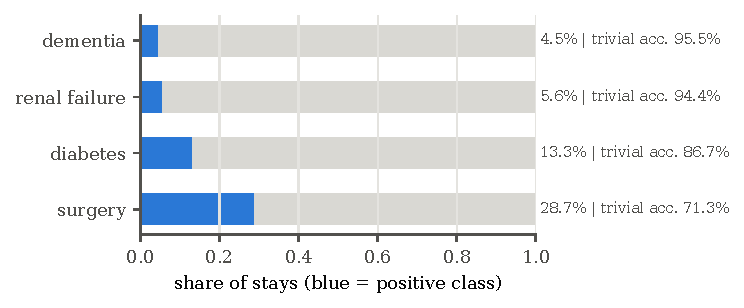
\includegraphics[width=0.62\linewidth]{fig1_prevalence.pdf}
\caption{Prevalence of the sensitive binary attributes in the reference database and accuracy of the trivial majority-class predictor.}
\label{fig:prev}
\end{figure}

\subsection{Individualisation}
On the unperturbed direct release, apparent uniqueness reaches \UniqDirZero{} at full knowledge and every isolation is correct (PPV \PpvDirZero, \cref{fig:so}). As soon as cells are shuffled, $U(k)$ becomes non-monotone: it rises with the first variables, then falls because the strict adversary loses the true record (\cref{prop:exact}). It ends at \UniqDirFifty{} for $\pi=50\%$. On the fully shuffled direct release, $U(k)$ still peaks at \UniqPeakDirHundred{} although no isolation designates the right person. Apparent uniqueness thus mostly measures the sparsity of the joint distribution, not the risk. The PPV separates the two situations: it stays close to 1 when few cells are shuffled and drops to about 0 at $\pi\ge 90\%$. At intermediate levels it rises with $k$ but is then computed on very few claims, so PPV must always be reported together with the number (or rate) of claims. Under bootstrap resampling, uniqueness is capped by duplicates and absences (\UniqSmpZero{} at $\pi=0$), whereas the PPV remains high (\PpvSmpZero).

\begin{figure}[t]
\centering
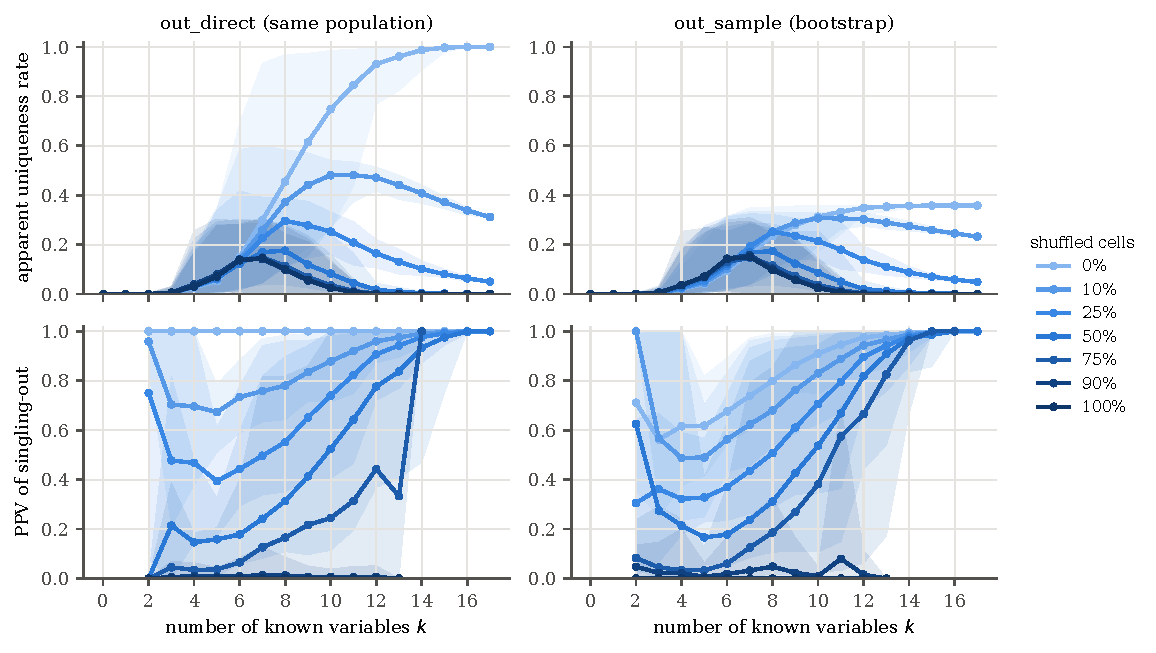
\includegraphics[width=\linewidth]{fig2_individualisation.pdf}
\caption{Individualisation knowledge curves (strict adversary). Top: apparent uniqueness rate. Bottom: positive predictive value of singling-out claims. Lines are means over \Norders{} revelation orders and bands are 2.5--97.5\% percentiles. Darker blue means more shuffling.}
\label{fig:so}
\end{figure}

\subsection{Linkability}
\Cref{fig:link} and \cref{tab:link} report linkage success. With exact matching, linkage at full knowledge falls from \LinkExDirZero{} ($\pi=0$) to \LinkExDirTen{} ($\pi=10\%$) and \LinkExDirTwentyFive{} ($\pi=25\%$). The tolerant adversary still links \LinkNNDirTen{} and \LinkNNDirTwentyFive{} of targets, and \LinkNNDirFifty{} at $\pi=50\%$. The strict adversary therefore underestimates the risk of perturbed releases by an order of magnitude. On bootstrap releases, raw linkage cannot exceed the presence ceiling ($L^\ast\approx\CeilSmp$). Once corrected (\cref{eq:kappaL}), $\kL$ reaches \KappaSmpZero{} at $\pi=0$, comparable to the direct release (\KappaDirZero). The two families can thus be compared on a common scale.

\begin{figure}[t]
\centering
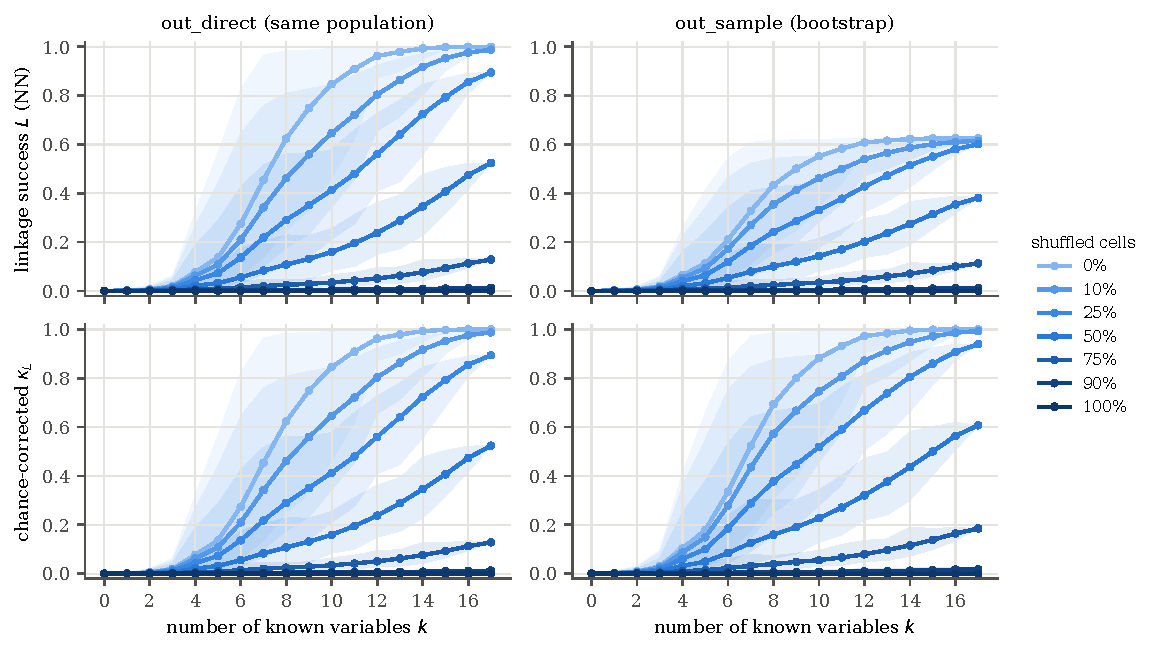
\includegraphics[width=\linewidth]{fig3_linkability.pdf}
\caption{Linkability knowledge curves (tolerant adversary). Top: expected linkage success $L$. Bottom: chance- and ceiling-corrected index $\kL$.}
\label{fig:link}
\end{figure}

\begin{table}[t]
\centering\small
\caption{Individualisation and linkability at full knowledge ($k=\kmaxA$). $U$: apparent uniqueness; PPV: precision of singling-out claims; $L_\text{ex}$, $L_\text{NN}$: linkage success of the strict and tolerant adversaries; $\kL$: corrected linkage index; nAUKC of $\kL$ over $k=1..\kmaxA$.}
\label{tab:link}
\begin{tabular}{@{}llrrrrrr@{}}
\toprule
Release & $\pi$ (\%) & $U$ & PPV & $L_\text{ex}$ & $L_\text{NN}$ & $\kL$ & nAUKC($\kL$) \\
\midrule
\csname @@input\endcsname tables/tab_individualisation_linkage.tex
\bottomrule
\end{tabular}
\end{table}

\subsection{Inference}
\Cref{fig:infdem} illustrates the accuracy paradox for dementia. On the fully shuffled direct release, accuracy at full knowledge is \InfDemAccDirHundred, below the trivial level of $1-p$, and decreases as knowledge increases, exactly as predicted by \cref{prop:accuracy}. Meanwhile balanced accuracy (\InfDemBaDirHundred) and MCC (\InfDemMccDirHundred) stay at their null values. Conversely, at $\pi=25\%$ accuracy (\InfDemAccDirTwentyFive) looks barely different from the trivial rule, whereas MCC (\InfDemMccDirTwentyFive) and AUPRC gain (\InfDemApDirTwentyFive) reveal a substantial leak. At $\pi=50\%$ the two families of scores even disagree in sign: raw accuracy is below the majority-class rule for dementia ($\Delta$Acc $=\InfDemAccGainDirFifty$) and diabetes ($\Delta$Acc $=\InfDiaAccGainDirFifty$), which would suggest that the release leaks nothing, whereas the MCC is \InfDemMccDirFifty{} and \InfDiaMccDirFifty{}, respectively. Across shuffling levels diabetes behaves like dementia (MCC \InfDiaMccDirTwentyFive{} at $\pi=25\%$, \InfDiaMccDirHundred{} at $\pi=100\%$). \Cref{tab:inf} gives all attributes.

\begin{figure}[t]
\centering
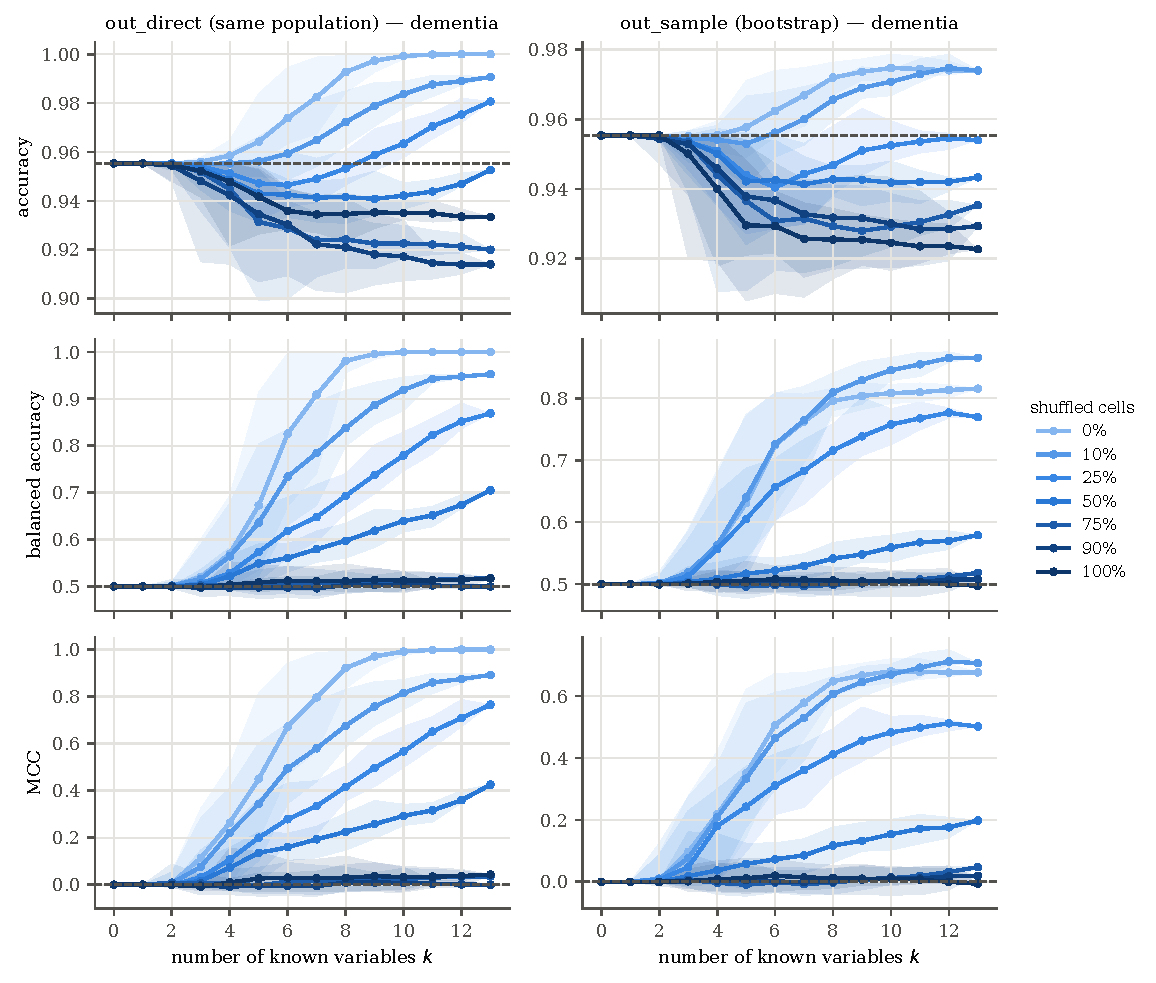
\includegraphics[width=\linewidth]{fig4_inference_demence.pdf}
\caption{Inference of dementia (prevalence \InfDemPrevDirZero) by the tolerant adversary. Dashed lines: trivial accuracy $1-p$, balanced accuracy $0.5$, MCC $0$. Raw accuracy falls \emph{below} the trivial level on uninformative releases (\cref{prop:accuracy}) and barely moves on informative ones, whereas MCC and balanced accuracy order the releases correctly.}
\label{fig:infdem}
\end{figure}

\begin{table}[t]
\centering\small
\caption{Attribute inference at full quasi-identifier knowledge ($k=\kmaxB$). $p$: prevalence; Acc: accuracy; $\Delta$Acc: gain over the majority class; BA: balanced accuracy; $\Delta$AP: AUPRC gain.}
\label{tab:inf}
\begin{tabular}{@{}lllrrrrrr@{}}
\toprule
Attribute & Release & $\pi$ (\%) & $p$ & Acc & $\Delta$Acc & BA & MCC & $\Delta$AP \\
\midrule
\csname @@input\endcsname tables/tab_inference.tex
\bottomrule
\end{tabular}
\end{table}

\subsection{Summary across releases}
\Cref{fig:heat} condenses every knowledge curve into its nAUKC. Raw accuracy rows are almost flat across shuffling levels (all values close to $1-p$) and are not even ordered at high $\pi$. The uniqueness row stays positive on fully shuffled releases, although no singling-out claim is correct there. The corrected rows ($\kL$, MCC, AUPRC gain) decrease with $\pi$ and reach $\approx0$ (within $\pm0.03$ Monte-Carlo noise) on the null releases. The nAUKC of $\kL$ falls from \AukcDirZero{} ($\pi=0$) to \AukcDirFifty{} ($\pi=50\%$) and \AukcDirHundred{} ($\pi=100\%$) on direct releases.

\begin{figure}[t]
\centering
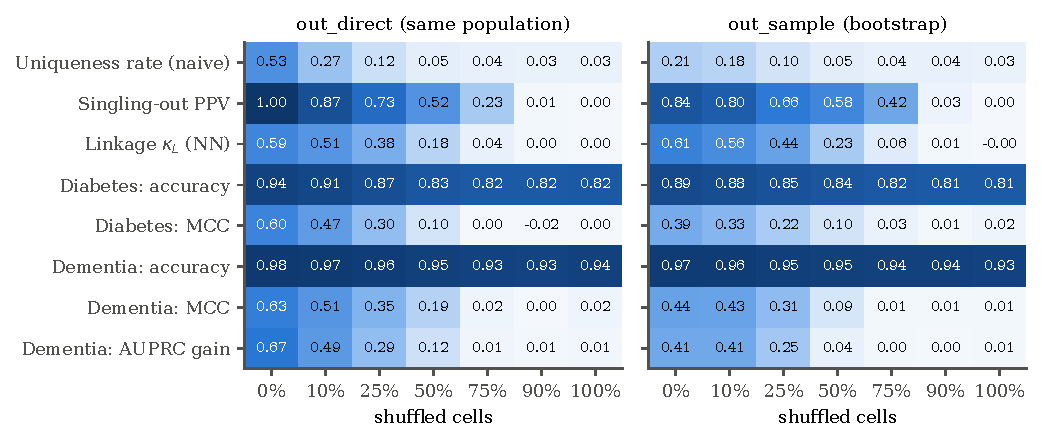
\includegraphics[width=\linewidth]{fig5_aukc_heatmap.pdf}
\caption{Normalised area under the knowledge curve (nAUKC) for naive and corrected indicators, by release family and shuffling level.}
\label{fig:heat}
\end{figure}

%% ============================================================================
\section{Discussion}
\label{sec:discussion}

\paragraph{Principal findings}
Three widely used indicators gave misleading answers in an imbalanced health database: apparent uniqueness, exact-match linkage and raw inference accuracy. The failures are systematic and predictable (\cref{prop:accuracy,prop:exact}). Uniqueness confuses sparsity with identifiability. Exact matching treats any perturbation as protection. Accuracy rewards the majority class and can even fall below its trivial value. The corrected indicators avoid these artefacts: PPV of singling out, $\kL$, MCC, balanced accuracy and AUPRC gain, computed for a tolerant adversary. They decrease with the perturbation level, vanish on null releases and put direct and bootstrap releases on a common scale.

\paragraph{Implications for the \G{} / CNIL assessment}
The \G{} Opinion asks whether singling out, linkability and inference ``remain possible''~\cite{wp29_2014,cnil_g29}. Our results suggest four reporting rules for data controllers and data protection officers who evaluate synthetic or perturbed health data:
(i)~report risk as a function of adversary knowledge rather than at one arbitrary quasi-identifier set;
(ii)~evaluate a tolerant adversary, not only exact matching;
(iii)~never report raw accuracy for rare sensitive attributes, and use MCC or balanced accuracy together with AUPRC gain;
(iv)~correct linkage for chance and for the presence ceiling, and compare with a null release.
These rules agree with the 2025 consensus recommendation to favour attack-based membership and attribute disclosure metrics~\cite{pilgram2025consensus} and with the criticism of similarity metrics~\cite{ganev2025inadequacy,yao2025dcr}. They add to that work an explicit treatment of imbalance.

\paragraph{Relation to Anonymeter}
Anonymeter~\cite{giomi2023anonymeter} corrects attack success with a control set of records not used for generation. Our null-release correction plays a similar role when no hold-out set exists, which is the case for the files studied here and for many legacy releases. The knowledge-curve view and the imbalance-aware scores could be plugged into Anonymeter's attack modules.

\paragraph{Limitations}
First, results were obtained on a fictitious replica of the course database. Absolute values depend on the data. The qualitative artefacts follow from \cref{prop:accuracy,prop:exact} and should hold more generally. Second, the tolerant adversary uses unweighted agreement counts. A Fellegi--Sunter weighting~\cite{fellegi1969linkage} or a probabilistic model~\cite{rocher2019estimating} would be stronger, so our numbers are lower bounds on the risk. Third, the adversary does not exploit internal inconsistencies between nested columns, which could flag perturbed cells. Fourth, column-wise shuffling is a simple stand-in for real synthetic generators. Applying the indicators to deep generative models and to the Avatar method~\cite{guillaudeux2023avatar} is a natural next step. Finally, only binary sensitive attributes were studied. Multi-class extensions (specialty, discharge mode) can use the multi-class MCC.

\paragraph{Ethics and data protection}
No real patient data were used. Consistent with data minimisation, the implementation never uses the stay identifier or the code lists in the attack. The identifier serves only to score success, and only aggregate statistics are written to disk; no individual linkage table is produced.

%% ============================================================================
\section{Conclusion}
Measuring the \G{} criteria on imbalanced health data requires more than counting unique records or reporting accuracy. We proposed a compact, chance-corrected and imbalance-aware set of indicators computed along knowledge curves. It exposes artefacts of naive indicators and orders releases consistently. We recommend that synthetic health data be published with these curves.

%% ============================================================================
\section*{Data and code availability}
\label{sec:availability}
The Python code (data generator, attacks, indicators, figures and the macros used in this manuscript) is provided as supplementary material (\texttt{M2MIAS/}). Running \texttt{run\_all.sh} on the course files regenerates every figure, table and number of this paper.

\section*{CRediT authorship contribution statement}
\textbf{Wajdi [Surname]:} Conceptualization, Methodology, Software, Formal analysis, Writing -- original draft. %% TODO: complete

\section*{Declaration of competing interest}
The authors declare that they have no known competing financial interests or personal relationships that could have appeared to influence the work reported in this paper.

\section*{Declaration of generative AI and AI-assisted technologies in the writing process}
During the preparation of this work the author(s) used Claude (Anthropic) to draft code and text. After using this tool, the author(s) reviewed and edited the content as needed and take(s) full responsibility for the content of the publication.

\section*{Acknowledgements}
The research question and data model were provided by the M2 MIAS project assignment of Pr Emmanuel Chazard (February 2026).

\bibliographystyle{elsarticle-num-names}
\bibliography{references}

\end{document}
